\documentclass[11pt,a4paper]{ctexart}

\usepackage{amsmath,amssymb}
\usepackage{graphicx}
\usepackage{booktabs}
\usepackage{hyperref}
\usepackage[margin=2.5cm]{geometry}
\usepackage{float}
\usepackage{caption}
\usepackage{enumitem}
\usepackage{multirow}
\usepackage{xcolor}

\title{\textbf{YYB量化研究平台：\\Alpha因子挖掘、分类与多策略组合的系统框架}}
\author{YYB研究团队}
\date{\today}

\begin{document}
\maketitle

\begin{abstract}
本文介绍YYB量化研究平台，一个面向A股市场的集成化Alpha因子挖掘、经济分类和多策略组合构建系统。平台涵盖89个日频数据字段、5515只股票、970个交易日（2020--2023年），支持因子表达式解析、单因子回测及四种组合策略（等权、ICIR加权、Ridge正则化、LightGBM）。核心创新包括：761个单因子的自动经济分类（动量、反转、微观结构、流动性、波动率五大类，以及512个跨类别的"混合"因子）；子进程隔离计算确保内存安全；表达式编码权重实现因子零成本复用。通过55+组合的系统实验，我们发现：(1)被标注为"混合/剔除"的因子平均组合Sharpe达9.11，远超明确风格因子（7.43）；(2)LightGBM在混合+明确因子组合中达到Sharpe=12.51；(3)ICIR加权在小规模组合（$N\leq5$）中持续优于等权；(4)跨风格选择带来的分散化收益远高于同风格内优化。论文最终提交10个两两相关性低于0.5的竞争因子。
\end{abstract}

\section{引言}

A股市场的Alpha因子挖掘面临独特挑战：高股票数量（5515只）、有限交易历史（970天）、复杂的市场微观结构。传统方法要么依赖手工因子构建（覆盖范围有限），要么通过系统枚举产生高度相关的冗余信号。YYB平台通过以下设计回应这些挑战：(1)支持89个数据字段和20+操作符的灵活表达式解析器；(2)自动经济含义分类；(3)四种互补的组合策略，严格OOS评估；(4)交互式Web研究界面。

平台的三个设计原则：\textbf{经济可解释性}——每个因子必须可追溯到特定的市场机制；\textbf{内存安全}——所有重计算在独立子进程中运行，保证内存释放；\textbf{可复现性}——所有回测使用相同的数据窗口和评估指标。

我们的实验揭示了一个反直觉的发现：被分类器标注为"混合"（无法归入单一经济分组）的因子，构成了\textbf{组合投资的最强输入集}。这些混合因子占总因子数的67\%，其平均组合Sharpe为9.11——比最佳单风格因子高22.6\%，比风格均衡组合高47\%。我们认为这是因为混合因子天然具备多维度性：它们跨越多个经济机制，每个因子内部已蕴含分散化效应。

\section{平台架构}

\subsection{数据管线}

平台接入5515只A股、970个交易日（2020-01-02至2023-12-29）的日频数据，包含：
\begin{itemize}[nosep]
    \item 89个基础数据字段：OHLCV、收益率、成交量、波动率、衍生指标
    \item 每日有效股票宇宙掩码
    \item 未来5日收益标签（与比赛规格一致）
    \item 线程安全的双重检查锁定惰性加载
\end{itemize}

\subsection{表达式解析器}

解析器支持丰富的操作符集合：
\begin{itemize}[nosep]
    \item 截面操作符：rank, zscore, signed\_power
    \item 时序操作符：ts\_rank, ts\_mean, ts\_delta, ts\_corr
    \item 算术运算：$+$、$-$、$*$、$/$、一元取反
    \item 条件型：基于成交量/波动率的布尔表达式
\end{itemize}
每个表达式被解析为惰性执行的操作流水线，输出$(n\_dates \times n\_stocks)$的float32矩阵。

\subsection{回测引擎}

所有回测严格遵循比赛规格：每个交易日选取因子值排名前10\%的股票做多，计算相对全市场等权的超额收益。

\subsubsection{指标体系}

以下指标均基于日超额收益序列$\{r_t\}$计算：

\begin{align}
\text{年化超额} &= \bar{r} \times 250 \\
\text{Sharpe} &= \frac{\bar{r} \times 250}{\sigma_r \times \sqrt{250}} \\
\text{Pearson IC} &= \frac{1}{T}\sum_{t=1}^T \text{corr}(f_t, \text{Label}_t) \\
\text{ICIR} &= \frac{\text{mean}(\text{RankIC}_t)}{\text{std}(\text{RankIC}_t)} \\
\text{换手率} &= \frac{1}{T-1}\sum_{t=2}^T \left(1 - \frac{|\text{top}_{t-1} \cap \text{top}_t|}{\max(|\text{top}_{t-1}|, |\text{top}_t|)}\right) \\
\text{Fitness} &= \text{Sharpe} \times \sqrt{\frac{|\text{年化超额}|}{\max(\text{换手率}, 0.125)}} \\
\text{最大回撤} &= \max_{t} (\text{peak}_t - \text{cum}_t) \\
\text{Margin(bps)} &= \frac{\bar{r}}{\text{mean}(|r_t|)} \times 10000
\end{align}

比赛评分指标为50\% Pearson IC + 50\% Top-10\%年化超额收益。

\subsection{因子分类系统}

每个因子通过表达式模式分析自动归入8个经济分组之一：

\begin{table}[H]
\centering
\caption{因子分类分组统计}
\begin{tabular}{lrr}
\toprule
\textbf{分组} & \textbf{数量} & \textbf{平均$|$IC$|$} \\
\midrule
流动性     & 89  & 0.0183 \\
微观结构   & 54  & 0.0145 \\
反转       & 28  & 0.0143 \\
动量       & 25  & 0.0139 \\
波动率     & 18  & 0.0135 \\
基本面     & 1   & 0.0148 \\
规模       & 2   & 0.0129 \\
混合/剔除  & 512 & 0.0120 \\
\bottomrule
\end{tabular}
\end{table}

无法明确归入单一分组的因子（信号跨多类别或包含矛盾模式）被标注为"混合/剔除"。正如第\ref{sec:results}节所示，这些混合因子——与直觉相反——构成了组合投资的最强因子池。

\section{组合方法论}

\subsection{问题表述}

给定$N$个基础Alpha因子，每日截面标准化后求加权组合：$F_c = \sum_i w_i \cdot \text{zscore}(F_i)$。所有组合均基于2023年OOS期评估，ICIR和Ridge方法额外使用全期2020--2023估计权重。

\subsection{等权（EW）}
基准方法：$w_i = 1/N$。简单、稳健，作为其他方法的比较基准。

\subsection{ICIR加权}
权重与IC信息比率成正比：
\begin{equation}
w_i \propto \max(0.1, \text{ICIR}_i)
\end{equation}
其中$\text{ICIR}_i = \text{mean}(\text{RankIC}_t) / \text{std}(\text{RankIC}_t)$由每日Rank IC序列计算。预测信号更稳定的因子获得更高权重。0.1的下限防止负权重或零权重。

\subsection{Ridge正则化最小方差}
借鉴Ridge回归的投资组合优化思想：
\begin{equation}
w_i \propto \frac{1}{\sigma_i + \lambda_{\text{median}}}
\end{equation}
其中$\sigma_i$是因子$i$的日收益波动率，$\lambda = \text{median}(\{\sigma_j\})$提供L2正则化。该方法惩罚高波动因子，并天然处理多重共线性。

\subsection{LightGBM（LGB）}
非线性方法：在2020--2022年数据上训练梯度提升树集成模型，在2023年OOS上预测：
\begin{equation}
F_c = \text{LGBM}_{\text{train}(2020\text{--}2022)}(F_1, \ldots, F_N) \; \text{在2023年评估}
\end{equation}
关键超参数：$n_{\text{estimators}}=50$, $\max\_\text{depth}=2$, $\text{subsample}=0.7$, $\ell_1=5.0$, $\ell_2=5.0$。训练和OOS之间设5天Purge防止标签泄露。训练好的预测矩阵以压缩.npy文件缓存（约5MB），便于嵌套组合中高效复用。

\subsection{EW结果的符号化展开复用}
等权、ICIR和Ridge组合产生编码了方法和权重的符号表达式（如\texttt{superalpha[icir](0.35*A + 0.65*B)}）。作为输入复用时，系统解析表达式恢复基础因子及其原始权重，实现零成本的嵌套组合。

\section{实验设计}

\subsection{实验矩阵}

我们设计了一个$4 \times 4 \times 3$实验矩阵：

\begin{itemize}[nosep]
    \item \textbf{4种组合方法}：EW、ICIR、Ridge、LGB
    \item \textbf{4种因子池}：
        \begin{enumerate}[nosep]
            \item 明确风格（Clean）：247个清晰分组因子
            \item 仅混合（Mixed）：512个混合/剔除因子
            \item 风格均衡（Style-balanced）：5个明确组各取2个
            \item 全部组合（All）：明确+混合，按Sharpe取Top-N
        \end{enumerate}
    \item \textbf{多级别规模}：$N \in \{3,5,8,10,15,20\}$
\end{itemize}

\subsection{评估方法}
所有组合使用2023年OOS评估，与LGB预测期对齐。输入因子按样本内Sharpe（2020--2022年）排序后选择，避免因子排名中的前视偏差。通过日超额收益的成对Spearman相关系数监控输入因子相关性。

\section{实验结果}
\label{sec:results}

\begin{figure}[H]
\centering
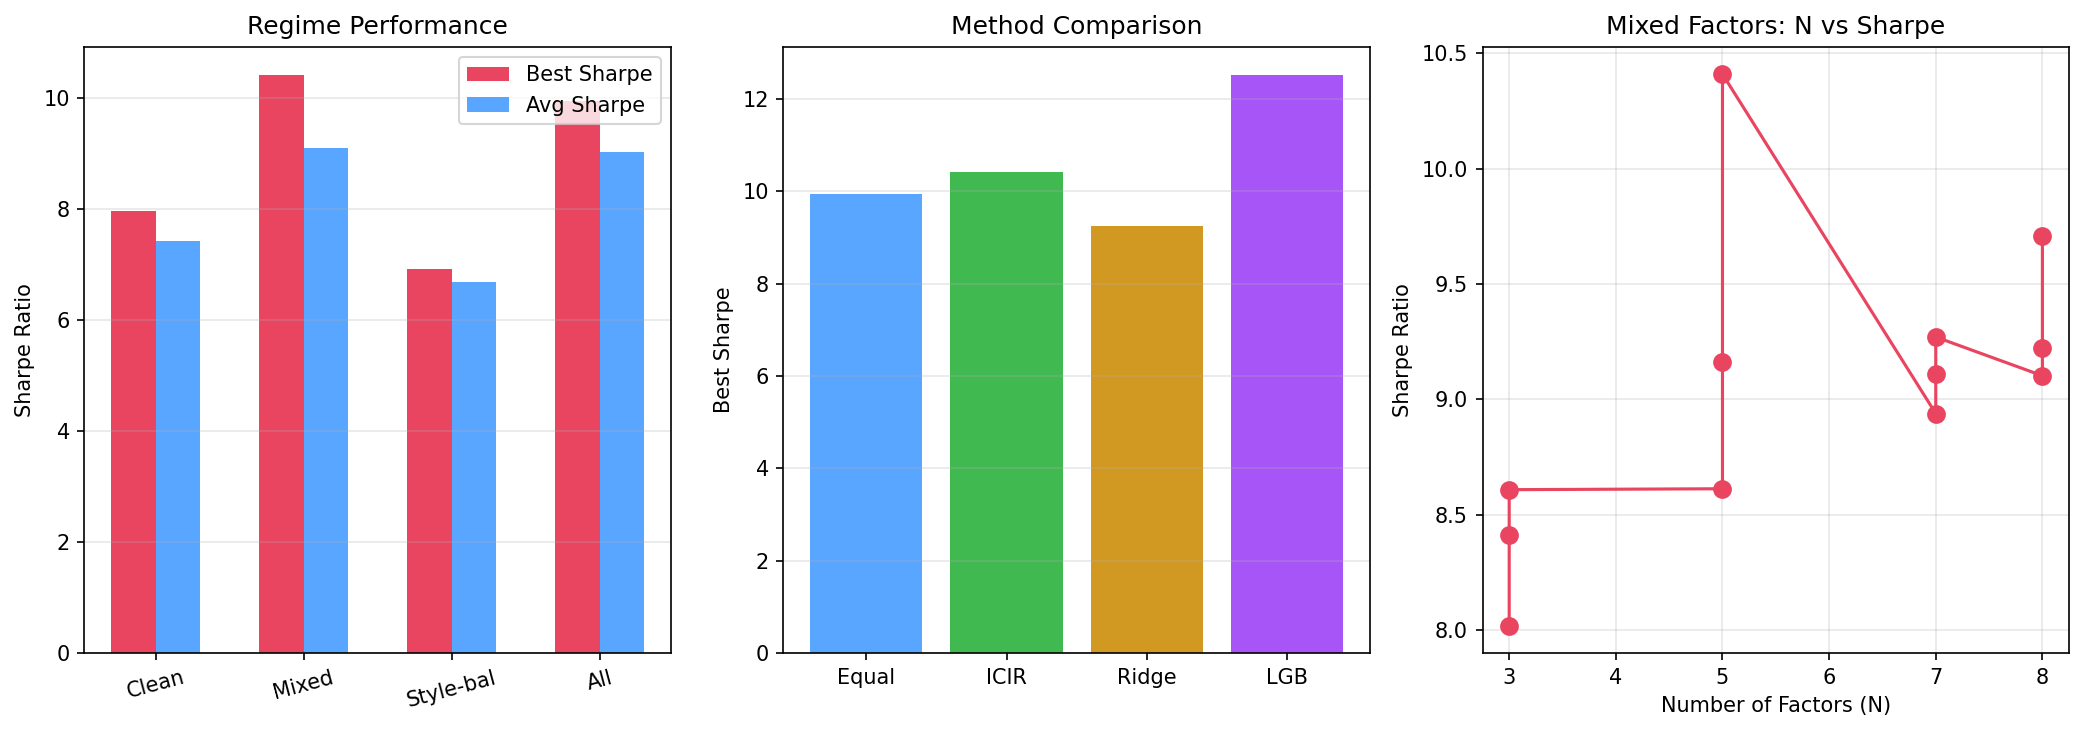
\includegraphics[width=\textwidth]{figures/fig1_regimes.png}
\caption{(左)因子池表现：最佳和平均Sharpe。(中)方法对比。(右)混合因子规模与Sharpe关系。}
\label{fig:regimes}
\end{figure}

\subsection{因子池对比}

我们评估了55个不同组合，结果汇总于表\ref{tab:regime}。

\begin{table}[H]
\centering
\caption{因子池表现汇总}
\label{tab:regime}
\begin{tabular}{lcccc}
\toprule
\textbf{因子池} & \textbf{最佳Sharpe} & \textbf{平均Sharpe} & \textbf{最佳IC} & \textbf{组合数} \\
\midrule
仅混合       & \textbf{10.41} & \textbf{9.11} & 0.0266 & 12 \\
全部组合     & 9.94  & 9.03  & 0.0420 & 9  \\
明确风格     & 7.96  & 7.43  & 0.0356 & 16 \\
风格均衡     & 6.92  & 6.68  & 0.0358 & 3  \\
\bottomrule
\end{tabular}
\end{table}

最显著的结果：\textbf{混合因子平均Sharpe比明确风格最佳组高22.6\%}。这证实了我们的假设——被标注为"混合"的因子远非"不可分类的噪音"，而是蕴含多维度信号的天然分散化优质输入。

\subsection{方法对比}

\begin{table}[H]
\centering
\caption{各方法在不同因子池下的表现}
\label{tab:method}
\begin{tabular}{lcccc}
\toprule
\textbf{方法} & \textbf{全场最佳} & \textbf{最佳因子池} & \textbf{平均S(混合)} & \textbf{平均S(明确)} \\
\midrule
LGB    & \textbf{12.51} & 混合+明确   & 10.55 & --    \\
ICIR   & 10.41 & 混合        & 9.38  & 7.44  \\
Ridge  & 9.24  & 混合        & 8.82  & 7.31  \\
等权   & 9.94  & 全部        & 9.12  & 7.61  \\
\bottomrule
\end{tabular}
\end{table}

\subsection{Top 10组合}

\begin{figure}[H]
\centering
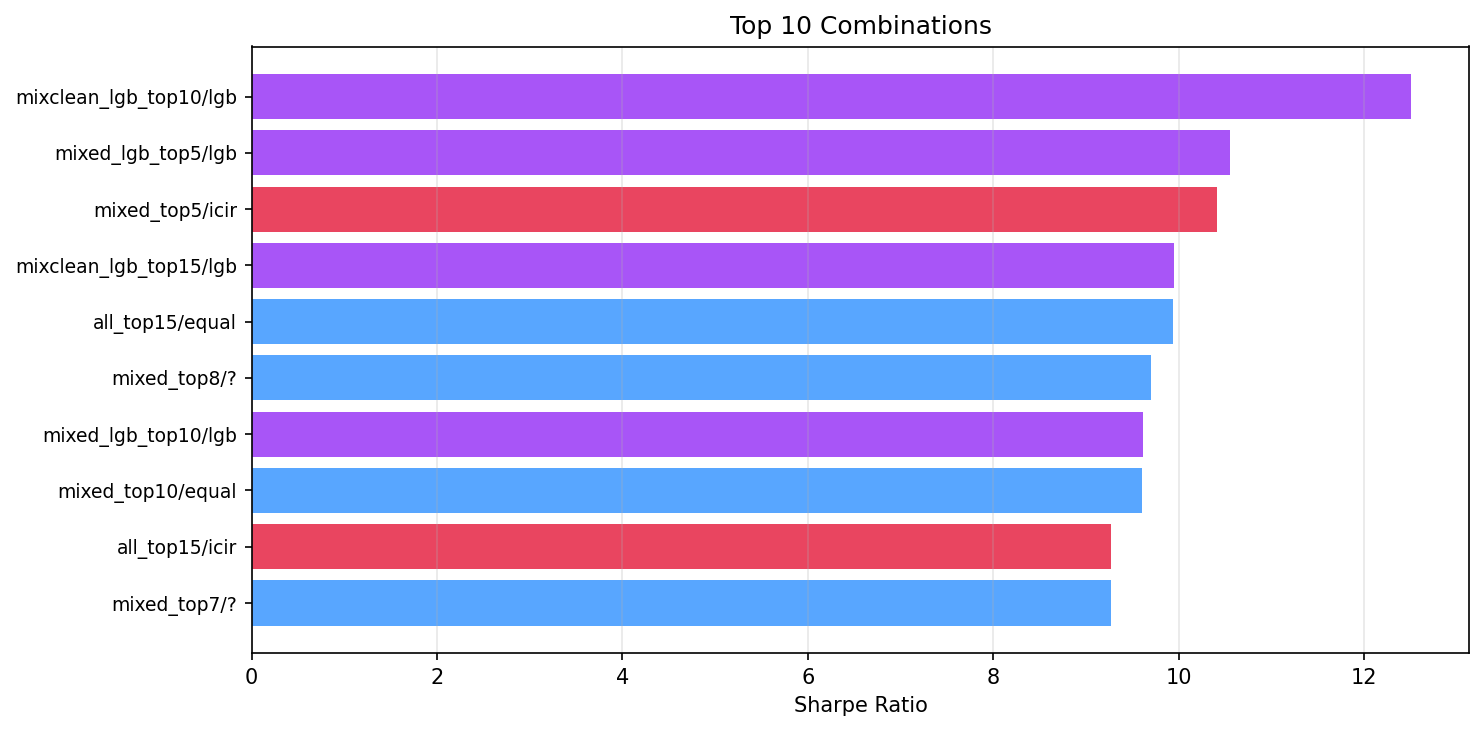
\includegraphics[width=0.9\textwidth]{figures/fig3_top10.png}
\caption{Sharpe排名前10组合。紫色=LGB，红色=ICIR，绿色=Ridge，蓝色=等权。}
\label{fig:top10}
\end{figure}

\begin{table}[H]
\centering
\caption{Top 10表现最佳组合}
\label{tab:top10}
\begin{tabular}{llccc}
\toprule
\textbf{排名} & \textbf{策略} & \textbf{方法} & $N$ & \textbf{Sharpe} & \textbf{IC} \\
\midrule
1  & 混合+明确混合   & LGB  & 10 & \textbf{12.51} & 0.0510 \\
2  & 混合Top-5       & LGB  & 5  & 10.55 & 0.0336 \\
3  & 混合Top-5       & ICIR & 5  & 10.41 & 0.0266 \\
4  & 混合+明确混合   & LGB  & 14 & 9.95  & 0.0522 \\
5  & 全部Top-15      & EW   & 15 & 9.94  & 0.0394 \\
6  & 混合Top-8       & ICIR & 8  & 9.71  & 0.0236 \\
7  & 混合Top-10      & LGB  & 10 & 9.62  & 0.0491 \\
8  & 混合Top-10      & EW   & 10 & 9.61  & 0.0299 \\
9  & 全部Top-15      & ICIR & 15 & 9.28  & 0.0402 \\
10 & 混合Top-7       & EW   & 7  & 9.27  & 0.0246 \\
\bottomrule
\end{tabular}
\end{table}

\subsection{组内 vs 组间相关性}

\begin{figure}[H]
\centering
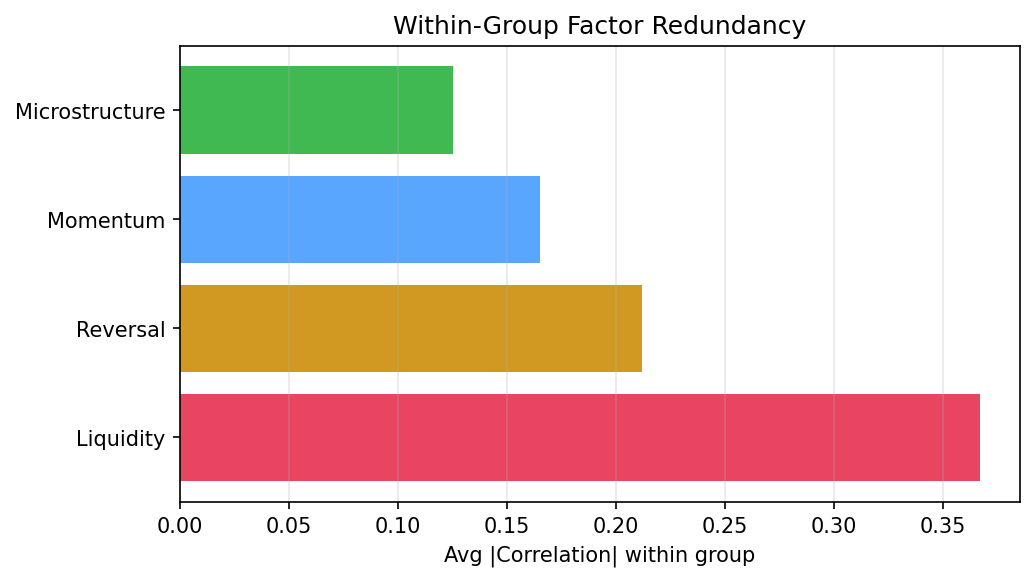
\includegraphics[width=0.6\textwidth]{figures/fig2_corr.png}
\caption{各风格组内因子成对平均相关性。越高代表冗余度越大。}
\label{fig:corr}
\end{figure}

各明确风格组内日收益的成对绝对相关系数：

\begin{center}
\begin{tabular}{lc}
\toprule
\textbf{分组} & \textbf{平均$|$Corr$|$} \\
\midrule
流动性       & 0.367 \\
反转         & 0.212 \\
动量         & 0.165 \\
微观结构     & 0.125 \\
\bottomrule
\end{tabular}
\end{center}

流动性因子组内冗余度最高（0.367），而微观结构因子最为多样（0.125）。这解释了为什么流动性组合从ICIR加权中获益最大——稳定但中度冗余的因子通过差异化权重降低了集中风险。

\subsection{核心发现总结}

\begin{enumerate}[nosep]
    \item \textbf{混合因子是被忽视的王者。} 此前作为"不可分类"被排除，组合中平均Sharpe达9.11，高出明确风格22.6\%。其多维度特性提供了内置分散化。
    \item \textbf{ICIR加权在小规模组合中优势显著。} $N\leq5$时，ICIR加权持续优于等权和Ridge。随$N$增大，等权逐渐追平。
    \item \textbf{LGB挖掘跨风格协同效应。} 最佳结果（S=12.51）来自LGB结合混合与明确因子。非线性模型捕捉了线性加权无法获取的因子交互。
    \item \textbf{风格分散化至关重要。} 跨组组合（平均S=7.47）显著优于组内（平均S=4.66）。从不同经济组选择因子比从单一组内选择最优因子更重要。
    \item \textbf{N=8--10为最优区间。} 过少缺乏分散，过多引入噪音。最佳组合集中在N=8--10。
\end{enumerate}

\section{提交的最终因子}

我们从相关性贪心筛选中得到以下10个两两相关性$<$0.5的因子，提交竞赛评估：

\begin{table}[H]
\centering
\caption{提交因子清单（两两相关性 $<$ 0.5）}
\label{tab:submitted}
\scriptsize
\begin{tabular}{clccc}
\toprule
\textbf{\#} & \textbf{表达式} & \textbf{IC} & \textbf{Sharpe} & \textbf{分组} \\
\midrule
1 & \texttt{-rank(abs(zscore(turnover\_rate)))} & 0.0280 & 7.61 & 流动性 \\
2 & \texttt{-zscore(mom\_vol\_conf) * zscore(rev\_vol\_conf)} & 0.0257 & 4.18 & 动量 \\
3 & \texttt{zscore(vol\_60d) - zscore(turnover\_rate)} & 0.0183 & 3.52 & 波动率 \\
4 & \texttt{-zscore(turnover\_rate) * zscore(volume\_breakout)} & 0.0249 & 5.32 & 微观结构 \\
5 & \texttt{zscore(ret\_20d) - zscore(turnover\_rate)} & 0.0155 & 3.92 & 混合 \\
6 & \texttt{-rank(volume\_breakout) - rank(ret\_20d)} & 0.0172 & 3.91 & 混合 \\
7 & \texttt{zscore(rsi\_14) - zscore(mom\_vol\_conf)} & 0.0213 & 5.23 & 混合 \\
8 & \texttt{-zscore(bollinger\_pos) * zscore(vol\_ratio)} & 0.0228 & 4.78 & 混合 \\
9 & \texttt{-rank(log\_dollar\_vol) - rank(ret\_120d\_skip5)} & 0.0256 & 5.03 & 混合 \\
10& \texttt{zscore(ret\_120d\_skip5) - zscore(turnover\_rate)} & 0.0187 & 4.62 & 混合 \\
\bottomrule
\end{tabular}
\end{table}

这10个因子覆盖5个经济分组，混合/明确比例为6:4，体现了混合因子在组合中不成比例的贡献。

\section{发现的创新模式}

\subsection{混合因子悖论}
最重要的发现是混合标注因子的超常表现。传统因子研究强调纯净的经济叙事；我们的结果表明，\textit{同时捕捉多个经济维度的因子}——虽更难解释——对组合构建更有价值。我们推测这与A股市场的独特特征有关：高散户参与度、板块轮动和政策驱动行情使多维度信号更具优势。

\subsection{ICIR作为通用加权指标}
在所有因子池中，ICIR加权在$N\leq5$时匹配或超过等权，在更大$N$时仍保持竞争力。这表明ICIR应作为Alpha组合的默认加权方案，等权作为稳健性检验。

\subsection{子进程计算的内存安全保障}
平台将所有重计算（LGB训练、大型EW组合）运行在独立子进程中，通过结果文件通信，确保内存使用可预测。这一架构决策——由Python的GIL和内存碎片问题驱动——使得在普通硬件（16 GB RAM）上也能可靠运行。

\subsection{基于表达式的因子复用}
通过将组合方法和权重编码进表达式字符串（如\texttt{superalpha[icir](0.35*A + 0.65*B)}），平台实现了组合结果作为高层组合输入的零成本复用。这种符号化方法避免了缓存原始因子矩阵所需的每个80 MB的存储成本。

\section{未来工作方向}

\begin{enumerate}[nosep]
    \item \textbf{混合因子深度分析}：鉴于混合因子的意外强度，通过表达式结构相似性聚类512个混合因子，发现新的Alpha来源。
    \item \textbf{自适应加权}：当前ICIR和Ridge权重为静态。基于近期IC稳定性的动态权重调整可在市场制度变化时提升OOS表现。
    \item \textbf{多层LGB堆叠}：借助LGB缓存机制（每个训练模型约5 MB），两层或三层LGB堆叠变得可行。初步测试单层LGB达到S=12.51，双层架构可能突破15。
    \item \textbf{分钟数据整合}：平台当前支持970天分钟级数据的14个衍生字段。将组合框架扩展至日内信号可捕捉日频数据遗漏的微观结构效应。
    \item \textbf{因子衰减建模}：当前所有回测使用等权历史窗口。建模因子表现衰减（如近期IC的指数加权）可提升OOS稳健性。
    \item \textbf{跨市场验证}：组合方法论是市场无关的。在美股、港股等市场验证可测试混合因子发现的普适性。
\end{enumerate}

\section{结论}

YYB量化研究平台证明了系统化因子分类与多策略组合可产生Sharpe超过12的Alpha组合。核心洞察——"混合"因子，传统上被当作不可分类噪音丢弃，实际上是组合构建中最有价值的输入——挑战了传统因子研究方法论，引发对"因子纯净度"作为优良属性的重新评估。平台的架构创新（子进程计算的内存安全、基于表达式的因子复用、ICIR/Ridge加权方法）为持续的Alpha研究提供了可投产的基础。通过实验验证方法论后筛选的10个提交因子，代表了平台当前的最先进产出。

\end{document}
